\chapter{المكدّسات و الطوابير (\textenglish{Stacks and Queues})}

لقد اكتشفنا مع القوائم المتسلسلة طريقة جديدة أكثر مرونة من الجداول لتخزين البيانات. هذه القوائم مرنة بشكل خاص لأنه يمكننا أن نُدرج فيها و نحذف منها بيانات من أي مكان أردنا و في أية لحظة.

المكدّسات و الطوابير التي سنكتشفها هنا هما شكلان خاصّان نوعاً ما من القوائم المتسلسلة. فهما تسمحان بالتحكّم بالطريقة التي تُضاف بها العناصر الجديدة إليها. هذه المرة لن نقوم بإضافة عناصر جديدة في وسط القائمة، بل فقط في البداية أو النهاية. 

المكدّسات و الطوابير تعتبران مفيدتان للغاية من أجل البرامج التي تحلل المعطيات الّتي تصل بالتدريج. سنرى بالتفصيل كيف تعملان في هذا الفصل.

تتشابه المكدّسات و الطوابير كثيراً، لكنهما تختلفان اختلافاً بسيطاً ستتعرف عليه بسرعة. سنكتشف أولاً المكدّسات و التي ستذكّرك بالقوائم المتّصلة بشكل كبير. 

بشكل عام، سيكون هذا الفصل بسيطاً إذا كنت قد فهمت جيّداً كيفية عمل القوائم المتسلسلة. إن لم تكن هذه حالتك، فأعد قراءة الفصل السابق لأننا سنحتاج إليه.

\section{المكدّسات (\textenglish{Stacks})}

تخيّل مكدّساً للقطع النقدية (الصورة التالية). يمكنك إضافة قطع أخرى واحدة تلو الأخرى في أعلى المكدّس، و يمكنك أيضاً نزع القطع من أعلى المكدّس. بالمقابل، لا يمكن نزع قطعة من أسفل المكدّس. إن أردت التجريب، أتمنى لك حظًاً موفّقاً !

\begin{figure}[H]
	\centering
	
\includegraphics[height=0.2\textheight]{Chapter_IV-2_Money-stack}
\end{figure}

\subsection{كيفية عمل المكدّسات}

مبدأ عمل المكدّسات في البرمجة ينصّ على تخزين البيانات مع وصولها على التوالي واحدة فوق الأخرى لكي نستطيع استرجاعها فيما بعد. مثلا، تخيّل مكدّساً للأعداد الصحيحة من نوع 
\InlineCode{int}
(الصورة الموالية). لو أضيف عنصراً (نتكلّم عن
\textbf{التكديس})،
فستتم إضافته في أعلى المكدّس، تماماً كما في لعبة 
\textenglish{Tetris} :

\begin{figure}[H]
	\centering
	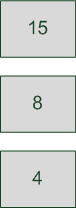
\includegraphics[height=0.2\textheight]{Chapter_IV-2_Stack}
\end{figure}
\begin{figure}[H]
	\centering
	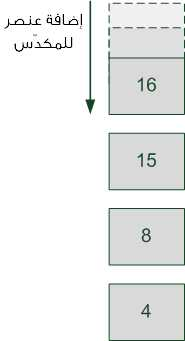
\includegraphics[height=0.3\textheight]{Chapter_IV-2_Stack-add}
\end{figure}

الأكثر أهمية هو وجود عملية تقوم باستخراج الأعداد من المكدّس. نحن نتكلّم عن
\textbf{إلغاء التكديس}.
نسترجع القيم واحدة تلو الأخرى، بدءً من الأخيرة الموضوعة أعلى المكدّس (الصورة الموالية). ننزع البيانات على التوالي حتى نصل إلى قاع المكدّس.

\begin{figure}[H]
	\centering
	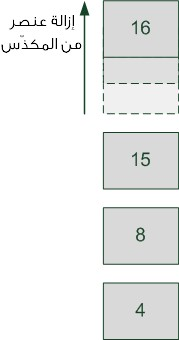
\includegraphics[height=0.3\textheight]{Chapter_IV-2_Stack-remove}
\end{figure}

نسمي هذا بخوارزمية
\textbf{\textenglish{LIFO}}،
و التي تعني
"\textenglish{Last In First Out}".
الترجمة : "آخر عُنصر تمت إضافته، هو أول عنصر يخرج".

عناصر المكدّس مرتبطة ببعضها بطريقة القوائم المتسلسلة. فهي تحمل مؤشّراً نحو العنصر الموالي و لا تتموضع بالضرورة بجنب بعضها في الذاكرة. يجب على آخر عُنصر (في أقصى أسفل المكدّس) أن يؤشّر نحو
\InlineCode{NULL}
لكي يقول أنّنا \dots لمسنا القاع :

\begin{figure}[H]
	\centering
	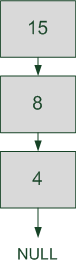
\includegraphics[height=0.2\textheight]{Chapter_IV-2_Stack-numbers}
\end{figure}

\begin{question}
 فيما ينفع كلّ هذا، واقعيّا ؟
\end{question}

توجد برامج تحتاج فيها إلى تخزين اليبانات مؤقّتاً لإخراجها اعتماداً على ترتيب محدد : يجب على آخر عُنصر أدخلته أن يخرج هو الأول.

لأعطي مثالاً واقعياً، يستعمل نظام التشغيل في حاسوبك هذا النوع من الخوارزميات لكي يتذكر الترتيب الذي تم استدعاء الدوال فيه. تخيّل مثالا :

\begin{enumerate}
	\item يبدأ البرنامج بالدالة
	\InlineCode{main}
	(مثل كل مرّة).
	\item تستدعي فيها الدالة 
	\InlineCode{play}.
	\item تقوم هذه الدالة 
	\InlineCode{play}
	بدورها باستدعاء الدالة
	\InlineCode{load}.
	\item ما إن تنتهي الدالة
	\InlineCode{load}،
	نعود إلى الدالة
	\InlineCode{play}.
	\item ما إن تنتهي الدالة 
	\InlineCode{play}،
	نعود إلى الدالة 
	\InlineCode{main}.
	\item أخيراً، ما إن تنتهي الدالة
	\InlineCode{main}.
	لا تبقى أية دالة تحتاج إلى الاستدعاء، ينتهي البرنامج.
\end{enumerate}

لكي "يتذكّر" الترتيب الذي تم فيه استدعاء الدوال، يُنشئ الحاسوب مكدّساً لهذه الدوال على التوالي :

\begin{figure}[H]
	\centering
	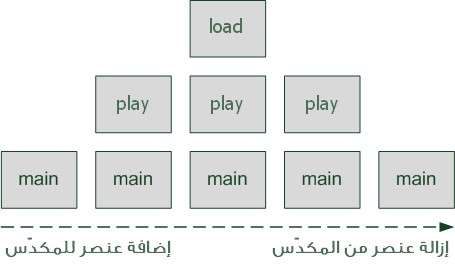
\includegraphics[width=0.6\textwidth]{Chapter_IV-2_Stack-history}
\end{figure}

هذا مثال واقعيّ عن استعمال المكدّسات. و بفضل هذه التقنية يعرف الجهاز الآن إلى أي دالة يجب عليه أن يعود. يمكنه أن يكدّس 100 استدعاء للدوال إن وجب الأمر، لكنّه سيرجع ليجد الدالة الرئيسية في أسفل المكدّس !

\subsection{إنشاء نظام مكدّس}

و الآن بما أننا فهمنا مبدأ عمل المكدّسات، فلنحاول بناء واحد. تماما مثل القوائم المتسلسلة، لا يوجد نظام مكدّس متضمّن في لغة الـ\textenglish{C}.
يجب أن ننشئه بأنفسنا.

سيكون لكل عنصر من المكدّس هيكل مماثل للهيكل الخاص بالقائمة المتسلسلة :

\begin{Csource}
typedef struct Element Element;
struct Element
{
	int number;
	Element *next;
};
\end{Csource}

يحتوي هيكل التحكّم على عنوان أول عنصر من المكدس، أي العنصر المتواجد في الأعلى :

\begin{Csource}
typedef struct Stack Stack;
struct Stack
{
	Element *first;
};
\end{Csource}

سنحتاج ككل إلى الدوال التالية :

\begin{itemize}
	\item تكديس  عنصر.
	\item إلغاء تكديس عنصر.
\end{itemize}

ستلاحظ أنه، على خلاف القوائم المتسلسلة، لا نتكلّم لا عن الإضافة و لا عن الحذف. نتكلّم عن التكديس و إلغاء التكديس. لأن هاتين العمليتين محدودتان على عنصر واحد محدد، كما رأينا. بهذا، يمكننا إضافة و نزع عنصر من المكدّس من الأعلى فقط.

يمكننا أيضاً كتابة دالة لإظهار محتوى المكدّس، أمر عمليّ للتأكد من أن البرنامج يعمل بشكل صحيح.

هيا بنا  !

\subsubsection{التكديس (\textenglish{stacking})}

يجدر بدالتنا
\InlineCode{stack}
أن تأخذ كمعاملين هيكل التحكّم في المكدّس (من نوع
\InlineCode{Stack})
و العدد الجديد لتخزينه.\\
أذكّرك بأننا نخزّن هنا أعداداً صحيحة
\InlineCode{int}،
لكن لا شيء يمنعنا من تعديل هذه الأمثلة لأنواع أخرى من البيانات. يمكننا تخزين أي شيء : أعداد
\InlineCode{double}،
محارف
\InlineCode{char}،
سلاسل محارف، جداول و حتى هياكل أخرى !

\begin{Csource}
void stack(Stack *stk, int newNumber)
{
	Element *new = malloc(sizeof(*new));
	if (stk == NULL || new == NULL)
	{
		exit(EXIT_FAILURE);
	}
	new->number = newNumber;
	new->next = stk->first;
	stk->first = new;
}
\end{Csource}

تتم الإضافة في بداية المكدّس لأنه، كما رأينا، يستحيل القيام بذلك في المنتصف. هذا مبدأ عمل المكدّسات، نضيف دائما من الأعلى. \\
بهذا، على عكس القوائم المتسلسلة، لا يجب أن ننشئ دالة لإدراج عنصر في منتصف المكدّس. يجب أن تكون الدالة
\InlineCode{stack}
هي الوحيدة الّتي يمكنها إضافة عناصر جديدة للمكدس.

\subsubsection{إلغاء التكديس (\textenglish{unstacking})}

دور دالة إلغاء التكديس هو حذف العنصر المتواجد في أعلى المكدّس، قد تشك في ذلك. لكن يجب على هذه الدالة أيضا أن تُرجع إلينا العنصر الذي حذفته. في حالتنا، هو العدد الّذي كان موجودا في أعلى المكدّس.

هذه هي الطريقة التي نصل بها إلى عناصر المكدّس : ننزعها واحداً تلو الآخر. نحن لا نتقدّم فيها باحثين عن الوصول إلى ثاني و ثالث عنصر. بل نطلب دائماً استرجاع على أول عنصر.

دالتنا
\InlineCode{unstack}
ستُرجع إذا
\InlineCode{int}
يوافق العدد المتواجد في رأس المكدّس  :

\begin{Csource}
int unstack(Stack *stack)
{
	if (stack == NULL)
	{
		exit(EXIT_FAILURE);
	}
	int unstackedNumber = 0;
	Element *unstackedElement = stack->first;
	if (stack != NULL§\footnotemark§ && stack->first != NULL)
	{
		unstackedNumber = unstackedElement->number;
		stack->first = unstackedElement->next;
		free(unstackedElement);
	}
	return unstackedNumber;
}
\end{Csource}

\begin{tcolorbox}[title={\footnotemark[1]ملاحظة مُرَاجِع الكتاب}, colback=orange!20, colframe=orange!70, fontupper=\small, coltitle=white, fonttitle=\normalsize, attach title]
يبدو لي أن مؤلّف الكتاب قد أضاف جزءً عديم الفائدة في الشرط الثاني :
\InlineCode{stack != NULL}،
فَبِوُصول البرنامج إلى ذلك السطر سيكون هذا الجزء من الشرط خاطئا بكلّ تأكيد لأنّنا قد تحقّقنا من عكسه في الشرط الأوّل 
(\InlineCode{if(stack == NULL)}).
و حتى عند عدم وجود الشرط الأوّل، فالتعليمة
\InlineCode{stack->first}
كانت ستعطّل البرنامج لأنّ مؤشّراً
\InlineCode{NULL}
لا يملك أيّة مركّبات !
\end{tcolorbox}

نسترجع العدد الذي في رأس المكدّس لنبعثه في نهاية الدالة. نعدّل عنوان أول عنصر من المكدّس بما أن هذا الأخير يتغير.
أخيراً، نحذف بالتأكيد رأس المكدّس القديم باستعمال
\InlineCode{free}.

\subsubsection{إظهار محتوى المكدّس}

بالرغم من أن هذه الدالة غير ضروريّة (الدالتان
\InlineCode{stack}
و 
\InlineCode{unstack}
كافيتان للتحكّم في المكدّس !)، ستكون مهمّة لاختبار عمل المكدّس و خاصّة "لمعاينة" النتيجة :

\begin{Csource}
void displayStack(Stack *stack)
{
	if (stack == NULL)
	{
		exit(EXIT_FAILURE);
	}
	Element *current = stack->first;
	while (current != NULL)
	{
		printf("%d\n", current->number);
		current = current ->next;
	}
	printf("\n");
}
\end{Csource}

بما أن هذه الدالة بسيطة بسخافة، فهي لا تحتاج شرحاً.

بالمقابل، حان الآن إذاً لكتابة الدالة الرئيسية لاختبار سلوك مكدّسنا :

\begin{Csource}
int main()
{
	Stack *myStack = initialization(); // See the previous chapter
	stack(myStack, 4);
	stack(myStack, 8);
	stack(myStack, 15);
	stack(myStack, 16);
	stack(myStack, 23);
	stack(myStack, 42);
	printf("\nStack's state :\n");
	displayStack(myStack);
	printf("I unstack %d\n", unstack(myStack));
	printf("I unstack %d\n", stack(myStack));
	printf("\nStack's state :\n");
	displayStack(myStack);
	return 0;
}
\end{Csource}

نُظهر حالة المكدّس بعد الكثير من التكديس و مرة أخرى بعد كثير من إلغاء التكديس. نُظهر أيضاً العدد الذي قُمنا بحذفه في كلّ مرة نقوم بإلغاء التكديس. النتيجة في الكونسول هي التالية :

\begin{Console}
Stack's state :
42
23
16
15
8
4

I unstack 42
I unstack 23

Stack's state :
16
15
8
4
\end{Console}

تأكّد أنك تفهم جيّداً ما يحصل في البرنامج. إذا فهمت هذا، فقد فهمت كيفية عمل المكدّسات !

يمكنك تنزيل مشروع المكدّسات كاملاً لو أردت :

\url{http://www.siteduzero.com/uploads/fr/ftp/mateo21/c/piles.zip}

\section{الطوابير (\textenglish{Queues})}

تشبه الطوابير المكدّسات كثيراً، إلا أنها تعمل بالإتجاه المعاكس !

\subsection{كيفية عمل الطوابير}

في هذا النظام، يتم وضع العناصر الواحد بعدَ الآخر. أوّل عنصر يخرج من الطابور هو أول عنصر يدخل إليه. نتكلّم هنا عن خوارزمية 
\textenglish{FIFO} (\textenglish{First In First Out})،
و هذا يعني : "أول من يصل هو أول من يخرج".

تسهل المشابهة بالحياة اليوميّة. حينما تشتري تذكرة لمشاهدة السينما، تقف في طابور شبّاك التذاكر (الصورة الموالية). باستثناء إن كنت أحد إخوة بائع التذاكر، يجدر بك الوقوف في الطابور و انتظار دورك مثل كلّ الآخرين. أول الواصلين هو أول من تتم خدمته.

\begin{figure}[H]
	\centering
	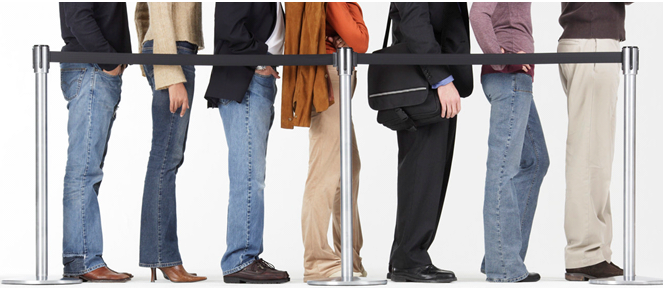
\includegraphics[width=0.8\textwidth]{Chapter_IV-2_Humans-queue}
\end{figure}

 في البرمجة، تفيد الطوابير في إيقاف مؤقّت للمعلومات حسب الترتيب الذي وصلت به. مثلاً، في برنامج مُحادثة، لو تتلقى ثلاثة رسائل يفصلها فارق زمني قصير جداً، يتم صفُّها في طابور واحدة تلو الأخرى في الذاكرة. ثم يتم إظهار أوّل رسالة وصلت ثم الثانية و هكذا.
 
يتم تخزين الأحداث التي تبعثها المكتبة
\textenglish{SDL}
التي قُمنا بدراستها أيضا في طابور. إذا حرّكت الفأرة، يتم توليد حدث من أجل كلّ بيكسل تحرّك فوقه مؤشّر الفأرة. تخزن الـ\textenglish{SDL}
الأحداث في طابور ثم تبعثها لنا واحدا واحدا في كلّ مرة نستدعي فيها الدالة
\InlineCode{SDL\_PollEvent}
(أو
\InlineCode{SDL\_WaitEvent}).

في لغة الـ\textenglish{C}.
الطابور هو قائمة متسلسلة أين يقوم كلّ عنصر فيها بالتأشير على العنصر الموالي، تماماً مثل المكدّسات. آخر عنصر من الطابور يؤشّر نحو
\InlineCode{NULL} :

\begin{figure}[H]
	\centering
	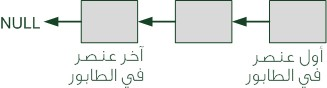
\includegraphics[width=0.5\textwidth]{Chapter_IV-2_Queue}
\end{figure}

\subsection{إنشاء نظام طابور}

نظام الطابور يشبه ذلك الخاص بالمكدّسات. يوجد اختلاف بسيط في كون أن العناصر تخرج في الإتجاه المعاكس، لا يوجد شيء صعب إن كنت قد فهمت المكدّسات.

سننشئ هيكل
\InlineCode{Element}
و هيكل تحكّم
\InlineCode{Queue} :

\begin{Csource}
typedef struct Element Element;
struct Element
{
	int number;
	Element *next;
};
typedef struct Queue Queue;
struct Queue
{
	Element *first;
};
\end{Csource}

تماما كالمكدّسات، كل عنصر من الطابور سيكون من نوع
\InlineCode{Element}.
بالإستعانة بالمؤشّر 
\InlineCode{first}
سنتوفّر دائماً على العنصر الأول و يمكننا من خلاله الصعود إلى آخر عنصر.

\subsubsection{إضافة عنصر إلى الطابور (\textenglish{enqueuing})}

الدالة التي تضيف عُنصُراً إلى الطابور تسمّى دالة "الإلحاق"
(\textenglish{enqueuing}).
توجد حالتان :

\begin{itemize}
	\item إما أن الطابور فارغ، في هذه الحالة يجب أن ننشئ الطابور بجعل المؤشّر
	\InlineCode{first}
	يؤشّر نحو العنصر الجديد الذي نحن بصدد انشائه.
	\item إما أن الطابور غير فارغ، في هذه الحالة يجب أن نتقدّم في الطابور إنطلاقاً من العنصر الأول حتى نصل إلى آخر عنصر. نضيف العنصر الجديد بعد آخر عنصر.
\end{itemize}
إليك ما يمكننا فعله عملياً :

\begin{Csource}
void enqueue(Queue *q, int newNumber)
{
	Element *new = malloc(sizeof(*new));
	if (q == NULL || new == NULL)
	{
		exit(EXIT_FAILURE);
	}
	new->number = newNumber;
	new->next = NULL;
	if (q->first != NULL) // The queue is not empty
	{
		// We move to the end of the queue
		Element *currentElement = q->first;
		while (currentElement->next != NULL)
		{
			currentElement = currentElement->next;
		}
		currentElement->next = new;
	}
	else /* The queue is empty, it's our first element */
	{
		q->first = new;
	}
}
\end{Csource}

ترى في هذه الشفرة المصدرية تحليل كلتا الحالتين، كلّ منهما يجب أن تتم دراستها على حدى. الاختلاف مقارنةً بالمكدّسات، و الذي يضيف لمسة صعوبة صغيرة، هو أنه يجب التموضع في نهاية الطابور لوضع العنصر الجديد. لكن لابأس فحلقة
\InlineCode{while}
كافية للقيام باللازم، هذا ما يمكنك ملاحظته.

\subsubsection{إزالة عنصر من الطابور (\textenglish{dequeuing})}

عملية إلغاء الإلحاق 
(\textenglish{dequeuing})
تشابه كثيراً عملية إلغاء التكديس. بامتلاكنا مؤشّرا نحو أول عنصر من الطابور، يكفي أن ننزعه و أن نُرجع قيمته.

\begin{Csource}
int dequeue(Queue *queue)
{
	if (queue == NULL)
	{
		exit(EXIT_FAILURE);
	}
	int dequeuedNumber = 0;
	// We verify if there's something to dequeue
	if (queue->first != NULL)
	{
		Element *dequeuedElement = queue->first;
		dequeuedNumber = dequeuedElement->number;
		queue->first = dequeuedElement->next;
		free(dequeuedElement);
	}
	return dequeuedNumber;
}
\end{Csource}

\subsubsection{حان دورك !}

تبقى دالة إظهار محتوى الطابور
\InlineCode{displayQueue}
و عملها مشابه لما قمنا به مع المكدّسات. سيسمح لك هذا بالتأكد من سلامة عمل الطابور.

قم بعد ذلك بكتابة
\InlineCode{main}
من أجل تجريب البرنامج. يجدر بنتيجة البرنامج أن تشبه هذه :

\begin{Console}
Queue's state :
4 8 15 16 23 42

I dequeue 4
I dequeue 8

Queue's state :
15 16 23 42
\end{Console}

يجدر أن تكون قادراً على إنشاء مكتبة الطوابير الخاصة بك، بملفات
\InlineCode{queue.h}
و
\InlineCode{queue.c}
مثلاً.

أقترح عليك تنزيل مشروع التحكّم في الطوابير كاملاً إن أردت. إنه يتضمّن الدالة
\InlineCode{displayQueue} :

\url{http://www.siteduzero.com/uploads/fr/ftp/mateo21/c/files.zip}

\section*{ملخّص}

\begin{itemize}
	\item تسمح المكدّسات و الطوابير بتنظيم معطيات في الذاكرة عند وصولها بالتوالي.
	\item تستعمل المكدّسات و الطوابير نظام قوائم متسلسلة لتجميع العناصر.
	\item في حالة المكدّسات، تتم إضافة المعطيات الواحدة فوق الأخرى. و إن أردنا استخراج بيانة، فسنستخرج آخر واحدة و التي كنا بصدد إضافتها (الأحدث). نتكّلم هنا عن خوارزمية 
	\textenglish{LIFO} (\textenglish{Last In First Out}).
	\item في حالة الطوابير، تتم إضافة المعطيات الواحدة بعد الأخرى. نقوم باستخراج البيانة الأولى و التي قمنا بإضافتها أولا للطابور (الأقدم). نتكلّم عن خوارزمية
	\textenglish{FIFO} (\textenglish{First In First Out}).
\end{itemize}
